
\section{实践}

\begin{frame}[fragile]{怎样使用\LaTeX{}得到一个PDF?}
	\begin{enumerate}
		\item 选择/编写 \LaTeX{}模板
		      \begin{itemize}
			      \item 通常直接下载给定的\LaTeX{}模板即可
		      \end{itemize}
		\item 编写文档内容
		      \begin{itemize}
			      \item 导入需要使用的包(可选)
			      \item 按\LaTeX{}语法组织内容,编写\LaTeX{}源文件
		      \end{itemize}
		\item 编译文件
		      \begin{itemize}
			      \item 使用\XeLaTeX{}等编译器对源文件进行编译
		      \end{itemize}
	    \item \alert{对照格式要求,检查最终的文件}
	\end{enumerate}
\end{frame}




\subsection{论文模板使用}
\begin{frame}[fragile]
	\frametitle{模板}
	\begin{itemize}
		\item<+-> 是什么?

		      \begin{itemize}
			      \item 设计好的格式框架
			      \item Word 中的样式:「学好 \LaTeX{} 可以更科学地使用 Word」
		      \end{itemize}

		\item<+-> 有哪些?

		      \begin{itemize}
			      \item 期刊:\pkg{revtex}、\pkg{elsarticle}、\pkg{IEEEtran}、\pkg{acmart}……
			      \item 学位论文:\pkg{thuthesis}、\pkg{ustcthesis}、\alert{\pkg{sustechthesis}}……
		      \end{itemize}

		\item<+-> 怎么用?
		      \begin{itemize}
			      \item |\documentclass{...}|,配置参数,照常编写
			      \item \alert{看文档,看文档,看文档}
		      \end{itemize}

		\item<+-> 去哪里找?

		      \begin{itemize}
			      \item CTAN \link{https://ctan.org} 或 GitHub \href{https://github.com}{\faGithub}
			      \item 期刊/会议官网
			      \item SUSTech LaTeX 模板目录 \link{https://github.com/SUSTC/latex-template}
			      \item 「U 盘拷给你的模板一定是过时的」
		      \end{itemize}
	\end{itemize}
\end{frame}


\begin{frame}{论文排版}
	\begin{itemize}
		\item 获取模板
		      \begin{itemize}
			      \item 随发行版自带、手动官网下载
			      \item 模板文档类 \texttt{.cls} 文件
			      \item 示例 \texttt{.tex} 文件
		      \end{itemize}
		\item 编辑 \texttt{.tex} 文件:添加用户内容
		\item 编译:生成 PDF 文档
	\end{itemize}
\end{frame}

\begin{frame}[fragile]{论文排版举例}
	\begin{exampleblock}{南方科技大学学位论文}
		\begin{itemize}
			\item 获取模板:github下载
			      \begin{itemize}
				      \item 打开\url{https://github.com/SUSTech-CRA/sustech-master-thesis/releases}
				      \item 下载最新版
				      \item 解压到某个文件夹(比如个人存论文的目录)
			      \end{itemize}
			\item 仔细阅读README
			\item 编辑 |sustechthesis-example.tex, sustech-setup.tex| 等源文件 
			\item 编译
			      \begin{itemize}
				      \item 运行命令|latexmk sustechthesis-example.tex|
			      \end{itemize}
		\end{itemize}
	\end{exampleblock}
\end{frame}


\begin{frame}{几种在作业/论文中常用的模版}
	\begin{columns}[c]
		\begin{column}{.45\textwidth}
			\begin{itemize}
				\item 毕业论文模版 \url{https://github.com/SUSTech-CRA/sustech-master-thesis}
				\item IEEE \url{https://template-selector.ieee.org/secure/templateSelector/publicationType}
				\item 同学制作的作业模板 \url{https://github.com/ziqin/LaTeX-SUSTechHomework}
			\end{itemize}
		\end{column}
		\begin{column}{.45\textwidth}
			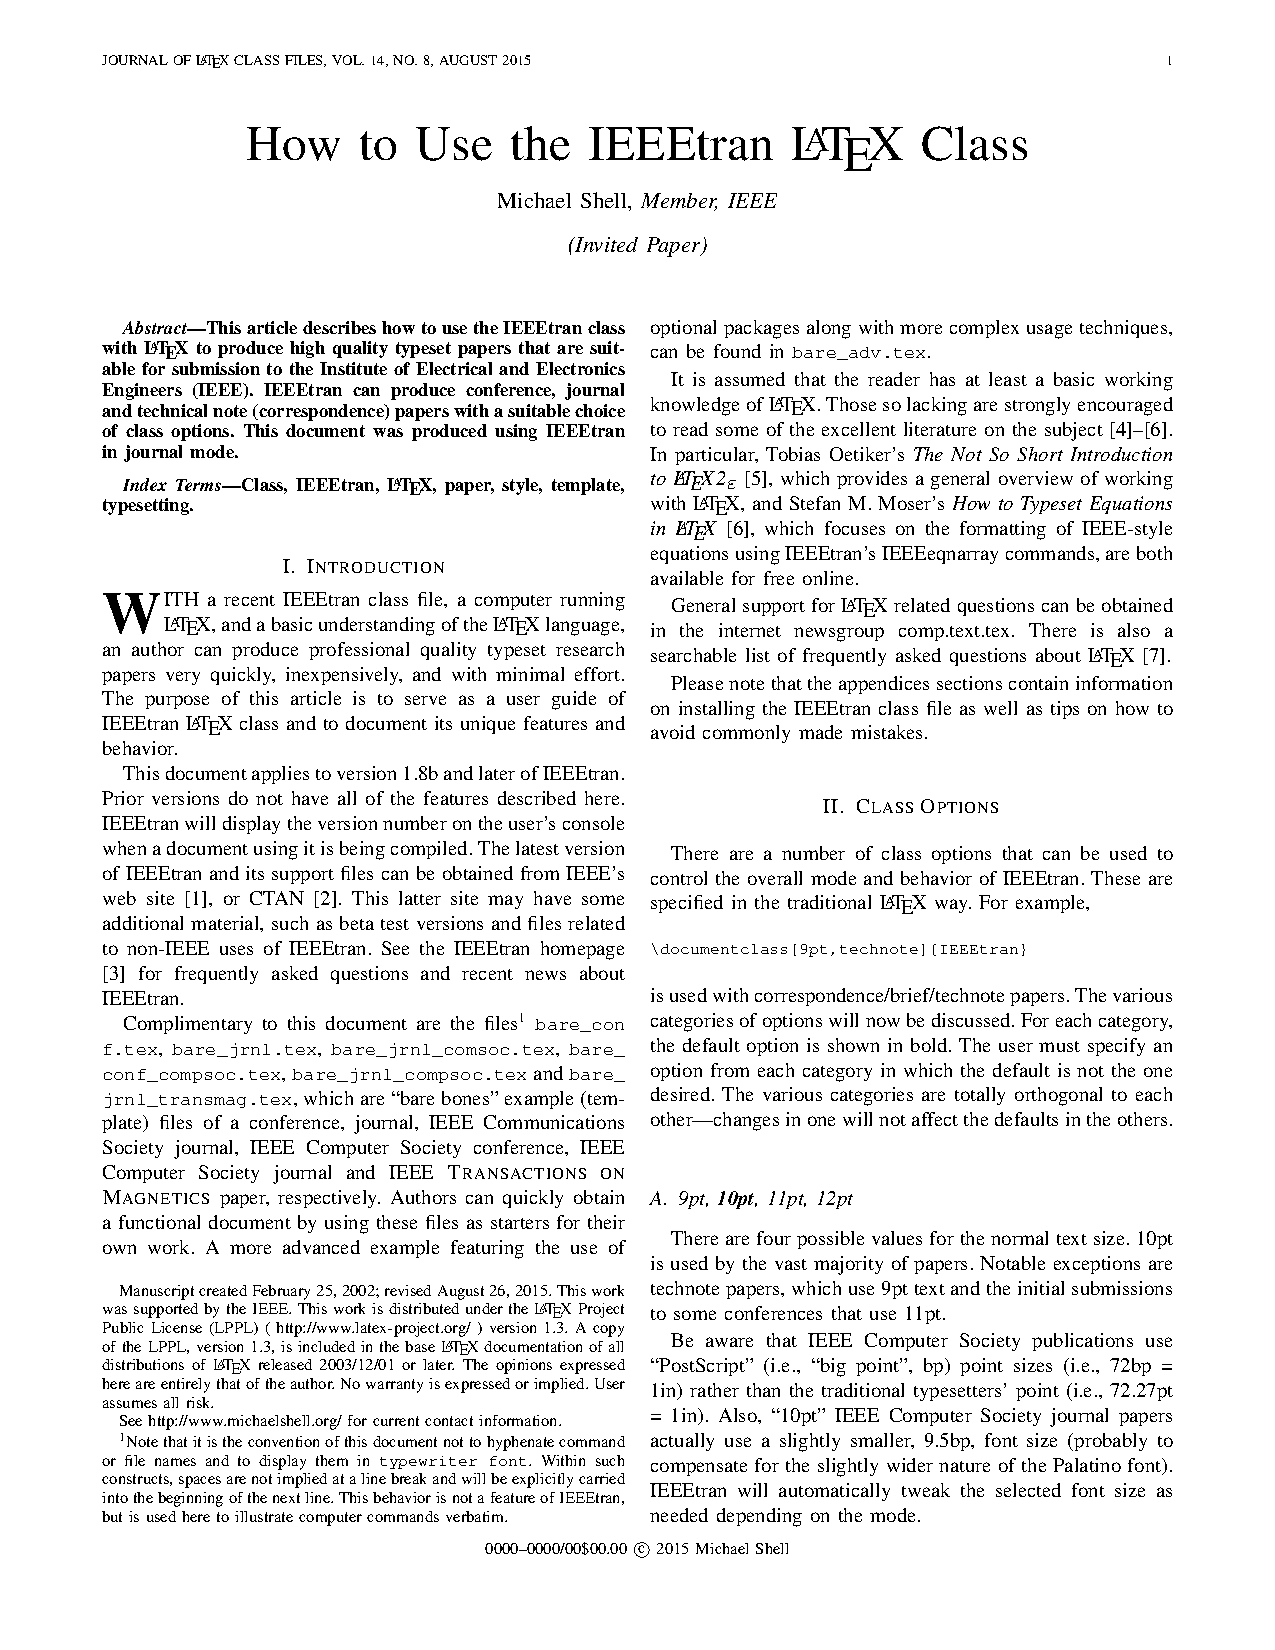
\includegraphics[width=0.75\textwidth]{docs/IEEE_template_1.pdf}
		\end{column}
	\end{columns}
\end{frame}


\subsection{本地安装,还是在线编辑?}


\begin{frame}[fragile]{选择发行版 -> 下载 -> 安装}
	\begin{itemize}
		\item Windows or Linux -> \texlive
		      \begin{itemize}
			      \item 下载 \texlive 离线安装镜像,每年 4月发布当年版本 \url{https://mirrors.sustech.edu.cn/CTAN/systems/texlive/Images/texlive.iso}
			      \item 解压或挂载下载的 ISO,运行 \rawcmd{install-tl-windows.bat} (Windows) or \rawcmd{install-tl} (Linux)
			      \item 切换默认仓库为国内镜像可加速今后升级,例如南科大镜像站 \url{https://mirrors.sustech.edu.cn/CTAN/systems/texlive/tlnet}
		      \end{itemize}
		\item macOS -> \mactex
		      \begin{itemize}
			      \item $\approx$ \texlive 在 Mac 下重新封装版本
			      \item 需要下载独立的安装包 \url{https://mirrors.sustech.edu.cn/CTAN/systems/mac/mactex/MacTeX.pkg}
		      \end{itemize}
	\end{itemize}
	\emph{不推荐安装 C\TeX 套装}
	\begin{itemize}
		\item \emph{存在严重 bug,并且完全过时(2012年已经停止维护)。}
	\end{itemize}
\end{frame}

\begin{frame}[fragile]{选择本地编辑器}
	\begin{itemize}
		\item<+-> 专用型
		      \begin{itemize}
			      \item TeXworks:\TeX{} Live 自带 \faWindows{} \faApple{} \faLinux{}
			      \item \emph{TeXstudio}:功能丰富,对新手友好 \faWindows{} \faApple{} \faLinux{}
			      \item TeXShop:Mac\TeX{} 自带 \faApple{}
			      \item WinEdt:功能丰富,收费 \faWindows{}
		      \end{itemize}

		\item<+-> 通用型

		      \begin{itemize}
			      \item \emph{Visual Studio Code}:借助插件 \pkg{LaTeX Workshop}  + \pkg{LaTeX Utilities}
			      \item Atom:听说很卡?
			      \item Sublime Text:收费
			      \item Vim:|q|、|q!|、|wq|、|wq!|
		      \end{itemize}

		\item<+-> 编辑器对比:\link{https://tex.stackexchange.com/q/339}
		      \link{https://en.wikipedia.org/wiki/Comparison_of_TeX_editors}
		      \link{https://www.zhihu.com/question/19954023}
	\end{itemize}
\end{frame}


\begin{frame}[fragile]{太麻烦!用在线的}

	\begin{itemize}
		\item 通过在线平台编辑、编译
		\item 免去安装/升级等一系列烦恼
		\item 可以多人协作
		\item 支持中文,但有时需要自己上传字体
	\end{itemize}

	\begin{itemize}
		\item Overleaf
		      \begin{itemize}
			      \item \url{https://www.overleaf.com}
		      \end{itemize}
		\item ShareLaTeX by 计算机研究协会
		      \begin{itemize}
			      \item \url{https://sharelatex.cra.moe/}
		      \end{itemize}
	\end{itemize}
\end{frame}

\subsection{LLM辅助工具}
\begin{frame}[fragile]{LLM辅助工具}
  现下各种大语言模型在我们编写\LaTeX{}过程中可以起很强的辅助作用。
  \begin{itemize}
    \item 这个宏包应该怎么用?
    \item 这个命令是什么意思?
    \item 这个环境的参数是什么?
    \item 怎么调整表格的复杂对齐?
    \item 为啥报错了?
  \end{itemize}
  \textcolor{red}{LLM是基于训练数据的概率模型,不保证100\%准确性!}
\end{frame}

\begin{frame}[fragile]{LLM问答实例}
  \begin{columns}[c]
		\begin{column}{.33\textwidth}
      \begin{exampleblock}{复杂表格格式设置}
        问:\\\quad tabularx 如何在固定列宽的同时设置左对齐和右对齐,同时允许单元格内自动换行?\\
        答:
        \begin{itemize}
          \item 如何控制宽度:……
          \item 如何左对齐:……
          \item 如何右对齐:……
          \item 如何混合对齐:……
          \item 如何自动换行:……
        \end{itemize}
      \end{exampleblock}
		\end{column}
		\begin{column}{.33\textwidth}
			\begin{exampleblock}{宏包使用教程}
        问:\\\quad LaTeX的caption宏包有什么用?\\
        答:\\\quad caption 宏包是……:
        \begin{itemize}
          \item 主要功能:……
          \item 基本用法:……
          \item 常用选项:……
          \item 示例代码:……
          \item 注意事项:……
        \end{itemize}
      \end{exampleblock}
		\end{column}
    \begin{column}{.33\textwidth}
			\begin{exampleblock}{报错原因查询}
        问:\\\quad LaTeX中以下报错是什么原因?……\\
        答:\\\quad 这个错误表明……。以下是修复后的代码:……\\
        \begin{itemize}
          \item 关键修改说明:……
          \item 替代方案:……
          \item 完整验证流程:……
          \item 常见错误排查:……
        \end{itemize}
      \end{exampleblock}
		\end{column}
	\end{columns}
\end{frame}


